\documentclass[draft,ras]{Template/AGUTeX}

\usepackage{graphicx}   % if you want to include graphics files
\usepackage{subfigure}
\usepackage{setspace}
\usepackage{amsxtra}
\usepackage{amsmath}
\usepackage{amssymb}
\usepackage{multirow}
\usepackage{bm}
\RequirePackage{lineno}
\linenumbers
% graphics path
\graphicspath{{Figs/}}

\authorrunninghead{SWOBODA ET AL.}
\titlerunninghead{3-D ISR}


\authoraddr{Corresponding author: J. P. Swoboda,
Department of Electrical \& Computer Engineering,
Boston University, 8 Saint Mary�s Street
Boston, MA 02215, USA.
(swoboj@bu.edu)}

\begin{document}

\title{Space-Time Ambiguity Function in 3-D ISR}
%%%%%%%%%%%%%% Author Info %%%%%%%%%%%%%%%%%%%%%%%%%%%%%%%%%%%%%
\authors{John Swoboda,\altaffilmark{1}
Joshua Semeter,\altaffilmark{1} Philip Erickson \altaffilmark{2}}

\altaffiltext{1}{Department of Electrical \& Computer Engineering,
Boston University, Boston, Massachusetts, USA.}
\altaffiltext{2}{Atmospheric Science Division,
MIT Haystack Observatory, Westford Massachusetts, USA.}
%%%%%%%%%%%%%% Abstract %%%%%%%%%%%%%%%%%%%%%%%%%%%%%%%%%%%%%

\begin{abstract}By leveraging electronically steerable phased array antenna technology, incoherent scatter radars (ISR) have now become full three-dimensional remote sensors for ionosphere plasmas. Currently these systems are operating in the high latitude region where the ionosphere is highly dynamic in both space and time. Because of the highly dynamic nature of the ionosphere in this region it is import to differentiate between artifacts and the true behavior of the plasma. Often the three dimension data is fitted in a spherical coordinate space and then the parameters are interpolated to a Cartesian grid. This and other sources of error could be impacting the reconstructions of the plasma parameters.

In this study we present a new way of analyzing 3-D dimension ISR through use of the space-time ambiguity function. This concept is similar to the range ambiguity function that is used in traditional ISR for scanning antenna systems but has been extended to all spatial dimension along with time as well.

The use of this new ambiguity function allow us to pose this problem in terms of a  linear inverse problem for the lags of the intrinsic plasma autocorrelation function. From this we can explore the impact of non-stationarity in the plasma parameters in both time and space. Along with showing possible artifacts we will begin to explore ways of reducing these artifacts.

\end{abstract}

%%%%%%%%%%%%%%  End of Abstract %%%%%%%%%%%%%%%%%%%%%%%%%%%%%%%%%%


\begin{article}

%%%%%%%%%%%%%% Intro %%%%%%%%%%%%%%%%%%%%%%%%%%%%%%%%%%%%%

\section{Introduction}
Incoherent scatter radar (ISR) systems have enabled researchers since the 1950's to explore the ionosphere \citep{gordon58}. Using methodology developed by Dougherty, Farley and others these systems can give measurements of electron density $N_e$, Ion temperature $T_i$, electron temperature $T_e$, Ion velocity $V_i$ and other plasma parameters \citep{dougherty:farley1960}, \citep{farleydougherty:ISR2}, \citep{hagfors1961}, \citep{doughteryfarley:ISR3}. These parameters are measured by fitting a nonlinear theoretic autocorrelation function (ACF) model derived from first principles physics to an estimated intrapulse time autocorrelation of the scattered radar signal \citep{Lehtinen1996435}. 
%This initial work showed the nonlinear relationship between the plasma parameters and the incoherent scatter autocorrelation function. 

As with any real world measurement method there is limit to the spatial and temporal resolution of ISR systems. This resolution is determined by the ability of the sensor to create independent measurements of the ACF in time and space of what is essentially a zero-mean complex Gaussian process. At space and time extents smaller then these resolutions the random process that the ACF is derived from is assumed to be stationary. In ISR literature the ambiguity function encapsulates the spatial resolution in the range dimension. This ambiguity emerges as a function of range and correlation lag due to the pulse modulation and the finite bandwidth of the receiver \citep{farley1969}. The time resolution is determined by how long it takes to average the autocorrelation function to reduce the variance of the estimate to a desired level.

%The hard target radar world also uses an ambiguity to analyze resolution but it is a function of time delay and Doppler mismatch. The CPI for a pulse doppler is like the time ambiguity. This ambiguity is tied to 

Because the assumption of stationarity at the level of the ambiguity function constrains the measurement and creates a blurring and other forms of artifacts due to the non-linear fitting of plasma parameters. In order to reduce the impact of these ambiguities number techniques have been developed. Some techniques include trying to reduce the extent of the ambiguity function by adjusting the waveform. Barker code wave forms are used in ISR but mainly for low altitude studies of the E-region due to the inability to form a spectrum from them. Another method for reducing the ambiguity in range is using alternating codes \citep{Sultzer1993}. %These codes though do reduce the amount of power returned from a specific volume of plasma.

Another set of techniques often shown in the literature focus on reducing the impact of the ambiguity function through post processing. The first method, full profile analysis, consists of fitting physical parameter values to entire range extent taking into account all of the correlations between all locations \citep{holt1992}, \citep{Lehtinen1989133}, \citep{Lehtinen:1997uh}, \citep{hysell2008}. This technique often places constraints on the physical parameters as in \citet{hysell2008}. Because the the relationship between the autocorrelation function and the lags are non-linear this method often yields algorithms that require a large amount computation to calculate the covariance matrices between all of the values.

The other set of post processing methods is deconvolution methods, such as in \citet{nikoukar2008}, treat the problem as a linear inverse problem of the lags. Method such as total-variations or Tikihonov regularization can be applied to the lags to try to fill in the missing information nation from the null space of the operator. These methods are easy to compute and can rely on a large body of knowledge from engineering communities that study linear inverse problems. 

Recently phased array technology has started to be leveraged by ISR community. The Advance Modular Incoherent Scatter Radar (AMISR) systems have already been deployed both at the Poker Flat Alaska (PFISR) and Resolute Bay Canada (RISR) \citep{amisr.site}. The EISCAT-3D project is currently being developed using phased array technology as well and will be capable of multistatic processing \citep{eiscat3ddesign}. These new systems are already being used to create three dimensional reconstructions of plasma parameters \citep{Semeter2009738}, \citep{Nicolls:2007ie}, \citep{dahlgren2012di},\citep{Dahlgren:2012dq}. 

There has been no formal derivation of an ambiguity function for all three spatial dimensions for these systems, although up until recently ISR systems, which only had dish antennas, could not mitigate the finite beam width effects. In a highly dynamic region like the high latitude ionosphere this lack of knowledge can be problematic. There are numerous phenomena such as polar cap patches that may be moving through the field of view at very high speeds \citep{dahlgren2012di}. This motion can cause an apparent expansion in the shape of the beams if one represents the beams in the frame of reference of the moving plasma.

These three-dimensional reconstructions often consist of taking the fitted parameters and then interpolating them to a Cartesian space from the system's natural spherical coordinate space \citep{Butler:2013ul}. The step of fitting the autocorrelation function to the theoretical functions to find the final plasma parameters is a non-linear operation. Because of this it is impossible to exactly predict the impact on the parameter values as different plasma populations move through the field of view of the radar. Alternatively it is possible to treat the formation of the autocorrelation estimates as a linear process with each lag as an independent channel \citep{nikoukar2008}.

In this publication we will develop a model for a full three dimensional space-time ambiguity function for 3-D ISR systems. This function can also be modified to show the ambiguity within the rest frame of the moving plasma. In the end this full three dimensional can be represented as kernel in a Fredholm integral equation like in Equation \ref{eqn:friedholm} with $f(s)$ being the lag of the autocorrelation function at a specific time and position. 

\begin{equation}
\label{eqn:friedholm}
g(t) = \int_a^b K(t,s) f(s) ds
\end{equation}

The impact of the three-dimensional ambiguity on moving plasma will be shown through simulation. This ISR simulator fully emulates the ISR data creation process at the IQ level. 

Lastly possible mitigation techniques will be explored. These mitigation techniques will borrow heavily from the image and signal processing literature.


%%%%%%%%%%%%%% Ambiguity Derivation%%%%%%%%%%%%%%%%%%%%%%%%%%%%%%%

\section{Space-Time Ambiguity}

In the ISR literature the measurement ambiguity along the range dimension is often referred to simply as the ambiguity function \citep{hysell2008}. This only shows the measurement ambiguity along the range $r$. Due to the three-dimensional imaging capability of phased array ISR systems we will define a new set of terminology to describe this more complicated measurement which is now imaging the ionosphere in three-dimensional coordinates $\mathbf{r}=[x,y,z]^T$. We will represent the sampled coordinates within the radar with $_s$ such as $\mathbf{r}_s$.

Specifically we will refer to the measurement ambiguity in the range dimension as the range ambiguity, $W(\tau,r_s,r)$. The measurement ambiguity in the elevation and azimuth angles will be referred to as the angular or cross range ambiguity $F(\theta_s,\phi_s,\theta,\phi)$, where $\theta$ is the physical elevation angle, $\phi$ is the physical azimuth angle, $\theta_s$ is the elevation angle that the radar is pointing at and $\phi_s$ is the azimuth angle that the radar is pointing at. The since these two functions are separable they can be multiplied together to form the full spatial ambiguity $K(\tau,\mathbf{r},\mathbf{r}_s)$. Lastly integration time for each measurement will be referred to the time ambiguity. Again like the full spatial ambiguity function we can multiply the space and time ambiguity functions to get the Space-Time ambiguity function which will be represented as $L(\tau,\mathbf{r}_s,t_s,\mathbf{r},t)$ .% Might want to go through math from the kernel stuff.

\subsection{Derivation}

In order to develop the space-time ambiguity we will use two different sets of time commonly known in radar literature as fast-time $n$ and slow-time $t$. Fast-time looks at time on the order of the radar systems A/D conversion while slow-time time is looking at time on the order of the system's pulse repetition interval \citep{richards:fundamentalsigproc}. We will use the same reference for fast-time but slow time will be the time it takes the plasma to change state and thus change the ACF.

In order to start we will first develop the range ambiguity which is due to the pulse shape and receiver filter on the ISR systems. If we look at data received by the ISR system at time $n$, with a wavenumber $\mathbf{k}$ and pulse shape $s(n)$, noted as $x(n)$ we can see that the received signal can be represented as the following

\begin{equation}
\label{eq:xt}
x(n) \propto h(n) \ast \int_{\mathbf{r}} e^{-j\mathbf{k} \cdot \mathbf{r}}  s(n-\frac{2r}{c}) n_e(\mathbf{r},n) d\mathbf{r},
\end{equation}

\noindent where $h(n)$ is the receiver filter, $n_e(\mathbf{r},n)$ is the electron density fluctuation.  Generally it is assumed that the pass band of the filter is larger then the bandwidth of the electron density fluctuation \citep{kudeki:notes}.  As such it can  be assumed that filter will only act on the the shape of the pulse. This will change Equation \ref{eq:xt} to the following:

\begin{equation}
\label{ex:xtaug}
x(n) \propto \ast \int_{\mathbf{r}} e^{-j\mathbf{k} \cdot \mathbf{r}}  a(n-\frac{2r}{c}) n_e(\mathbf{r},n) d\mathbf{r}
\end{equation}
\noindent where $a(n)= h(n) \ast s(n)$.   

When the autocorrelation of the signal is done we find the following formula, \citep{nikoukar2008}.  

\begin{equation}
\label{ex:acf1}
\langle x(n)x^*(n+\tau)\rangle = \int_{\mathbf{r'}}\int_{\mathbf{r}} e^{-2j \mathbf{k}\cdot \left(\mathbf{r}'-\mathbf{r} \right)}a(n-\frac{2r}{c})a^*(n+\tau-\frac{2r'}{c}) \langle n_e(\mathbf{r},n)n_e(\mathbf{r}',n+\tau)\rangle d\mathbf{r} d\mathbf{r}'
\end{equation}
 
\noindent where $r'$ is the magnitude of the vector $\mathbf{r}'$. We can make some simplifying assumption at this point that the space-time autocorrelation function of $n_e(\mathbf{r},t)$, $\langle n_e(\mathbf{r},n)n_e(\mathbf{r}',n+\tau)\rangle$, will vanish as the magnitude of $\mathbf{x} \equiv \mathbf{r}'-\mathbf{r} $ increases. Once the spatial correlation is removed we can rewrite Equation \ref{ex:acf1} as 
 
 \begin{equation}
 \label{ex:acf2}
 \langle x(n)x^*(n+\tau)\rangle = \int_{\mathbf{r}} a(n-\frac{2r}{c})a^*(n+\tau -\frac{2r}{c}) \int_{\mathbf{x}} e^{-2j \mathbf{k}\cdot \mathbf{x}} \langle n_e(\mathbf{r},n)n_e(\mathbf{x}+\mathbf{r},n+\tau)\rangle d\mathbf{x} d\mathbf{r}.
 \end{equation}
 
 The inner integral is a spatial Fourier transform evaluated at the wave number of the radar $\mathbf{k}$
 \begin{equation}
 \label{eq:spft}
 \langle |n_e(\mathbf{k},r,\tau)|^2\rangle \equiv  \int_{\mathbf{x}} e^{-2j \mathbf{k}\cdot \mathbf{x} } \langle n_e(\mathbf{r},b)n_e(\mathbf{x}+\mathbf{r},n+\tau)\rangle d\mathbf{x}.
 \end{equation}
 
 \noindent Equation \ref{ex:acf2} becomes
 
 \begin{equation}
 \langle x(n)x^*(n+\tau)\rangle = \int_{r} a(n-\frac{2r}{c})a^*(n+\tau -\frac{2r}{c}) \langle |n_e(\tau,\mathbf{k},\mathbf{r})|^2\rangle dr.
 \end{equation}
 %angle ambiguity
 %E_e(\phi,\psi)\text{dirc}_N(\frac{d_1}{\lambda}\sin\phi \cos\psi)\text{dirc}_K\left(\frac{d_2}{\lambda}\sin\phi\sin\psi\right)
 It should be noted that the term $ a(n)a^*(n+\tau)$ is the soft target ambiguity function.  If $n$ is replaced with $2r_s/c$ we can see that the this function represented as $W(\tau,r_s,r)$ \citep{nikoukar:thesis}.  In order to simplify notation we will represent $ \langle |n_e(\tau,\mathbf{k},\mathbf{r})|^2\rangle$, as $R(\tau,\mathbf{r})$. Assuming, for the moment, that $R$ only varies across the range dimension $r$ we can now represent this in the form of a Fredholm integral equation
 
 \begin{equation}
 \label{eqn:fredfirst}
 \langle x(2r_s/c)x^*(2r_s/c+\tau)\rangle = \int_{r} W(\tau,r_s,r) R(\tau,r) dr.
 \end{equation}
 
This function is in a way a lag dependent smoothing along the range dimension of $R(\tau,r)$. 
 
The spatial ambiguity across angle is determined by the antenna beam pattern. In phase array radars this beam pattern is ideally the array factor multiplied by the element pattern \citep{Balanis:2005:ATA:1208379}. The array factor is determined by a number of things including the element spacing in both x and y $(dx,dy)$ and the wave number of the radar, $k$. Making idealized assumptions with no mutual coupling and that the array elements are cross dipole elements AMISR systems will have the following array pattern for pointing angle ($\theta_s,\phi_s$),
 
 \begin{equation}
 \label{eqn:amisrpat}
F(\theta,\phi,\theta_s,\phi_s) = \frac{1}{2}(1+\cos(\theta)^2)\left[ \frac{1}{MN} \left(1+e^{j(\psi_y/2 + \psi_x)}\right)\frac{\sin((M/2) \psi_x)}{\sin(\psi_x)} \frac{\sin((N/2) \psi_x)}{\sin(\psi_x/2)}\right]^2,
 \end{equation}
 
 \noindent where $\psi_x = -k d_x(\sin\theta\cos\phi-\sin\theta_s\cos\phi_s)$, $\psi_y = -k d_y(\sin\theta\sin\phi-\sin\theta_s\sin\phi_s)$.


This spatial ambiguity is a separable function made up of the components of $W(\tau,r)$ and $F(\theta,\phi,\theta_s,\phi_s)$. These two functions can be combined by multiplying, creating the spatial ambiguity function  $K(\tau,\mathbf{r}_s,\mathbf{r})$, and then doing a volume integration. This will create radar system's estimate of the ACF which will be referred to as $\rho(\tau,\mathbf{r}_s)$,

 %\begin{equation}

 \begin{align}
  \label{eqn:volume}
\rho(\tau,\mathbf{r}_s) &= \int F(\theta,\phi,\theta_s,\phi_s)W(\tau,r_s,r) R(\tau,\mathbf{r}) dV,\\
	&= \int K(\tau,\mathbf{r}_s,\mathbf{r}) R(\tau,\mathbf{r})dV.
\end{align}
 %\end{equation}

A rendering of an example of this full ambiguity function for an uncoded long pulse and antenna pattern in (\ref{eqn:amisrpat}) for four beams can be seen in Figure \ref{fig:amb4}.

\begin{figure}
	\centering
	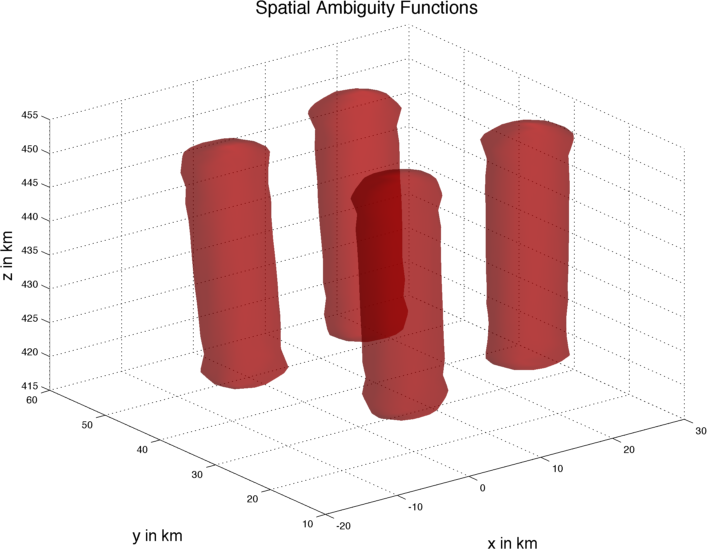
\includegraphics[width=5.5in]{spaceamb}
	\caption{Full Spatial Ambiguity Function}	
	\label{fig:amb4}
\end{figure}

Lastly, since the radar requires a finite amount of time to average pulses to create the estimate of the ACF we will add slow-time dependence to $R$. We will add another separable function $G(t_s,t)$ to the kernel,


\begin{align}
\label{eqn:sptamb}
\rho(\tau,\mathbf{r}_s,t_s) &= \int G(t_s,t)K(\tau,\mathbf{r}_s,\mathbf{r})R(\tau,\mathbf{r},t) dV dt\\
	\rho(\tau,\mathbf{r}_s,t_s) &=\int L(\tau,\mathbf{r}_s,t_s,\mathbf{r},t)R(\tau,\mathbf{r},t)dVdt.%\\
	%L(\tau,\mathbf{r}_s,t_s,\mathbf{r},t) &= G(t_s,t)F(\theta_s,\phi_s,\theta,\phi)W(\tau,r_s,r)
\end{align}

\noindent The final kernel, $L(\tau,\mathbf{r}_s,t_s,\mathbf{r},t)$ encompasses the full space-time ambiguity.

\subsection{Ambiguity after Frame Transformation}

We will now focus on the impact of the motion of plasma as it is going through the field of view of the radar. We will assume that the radar is integrating over a length of time $T$ beginning at $t_s$. The kernel $L$ will be represented as a separable function $K$ and $G$ as in (\ref{eqn:sptamb}). In this case $G$ will be an indicator function of length $T$ and centered at $t_0+1/2$. This will change (\ref{eqn:sptamb}) to the following,

\begin{equation}
\label{eqn:L2}
\rho(\tau,\mathbf{r}_s,t_s) = \int K(\tau,\mathbf{r}_s,\mathbf{r}) \int_{t_s}^{t_s+T}R(\tau,\mathbf{r},t) dt dV.
\end{equation}

Of specific interest are instances in the high latitude ionosphere where embedded plasma structures are moving due to the electric field of the magnetosphere. Because of this it will be assumed that the plasma is rigid object and will not deform with respect to $\mathbf{r}$ over time period $[t_0,t_0+T]$. Also it will be assumed that it will be moving with a constant velocity $\mathbf{v}$. Thus $R(\tau,\mathbf{r},t)\Rightarrow R(\tau,\mathbf{r}+\mathbf{v}t)$. At this point (\ref{eqn:L2}) becomes,

\begin{equation}
\label{eqn:L3}
\rho(\tau,\mathbf{r}_s,t_s) = \int \int_{t_s}^{t_s+T} K(\tau,\mathbf{r}_s,\mathbf{r})R(\tau,\mathbf{r}+\mathbf{v}t)dtdV\end{equation}

A change of variables where $\mathbf{r}' = \mathbf{r}+\mathbf{v}t$ acts as a Galilean transform and applies a warping to the kernel and changing the frame of reference. Then (\ref{eqn:L3}) becomes

\begin{equation}
\label{eqn:L4}
\rho(\tau,\mathbf{r}_s,t_s)= \int \int_{t_s}^{t_s+T} K(\tau,\mathbf{r}_s,\mathbf{r}'-\mathbf{v}t)R(\tau,\mathbf{r}')dtdV.
\end{equation}

\noindent Since $R(\tau,\mathbf{r}')$ is no longer dependent on $t$ (\ref{eqn:L4}) becomes,

\begin{equation}
\label{eqn:L5}
\rho(\tau,\mathbf{r}_s,t_s)= \int \left[ \;\; \int_{t_s}^{t_s+T}  K(\tau,\mathbf{r}_s,\mathbf{r}'-\mathbf{v}t)dt \;\; \right]R(\tau,\mathbf{r}')dV.
\end{equation}

By performing the integration in $t$ the problem can now be simplified further back to a Fredholm integral equation by simply replacing the terms  in the square brackets as a new kernel $A$,

\begin{equation}
\label{eqn:L6}
\rho(\tau,\mathbf{r}_s,t_s)= \int A(\tau,\mathbf{r}_s,t_s,\mathbf{r}') R(\tau,\mathbf{r}')dV.
\end{equation}

\noindent The impact of the plasma velocity on the ambiguity function can be seen in Figure \ref{fig:ambtime}. This is the same ambiguity as seen in Figure \ref{fig:amb4} but with a velocity of 500 m/s in the $y$ direction over a period of 2 minutes. This velocity creates a larger ambiguity function in the frame of reference of the moving plasma.
\begin{figure}[!t]
	\centering
	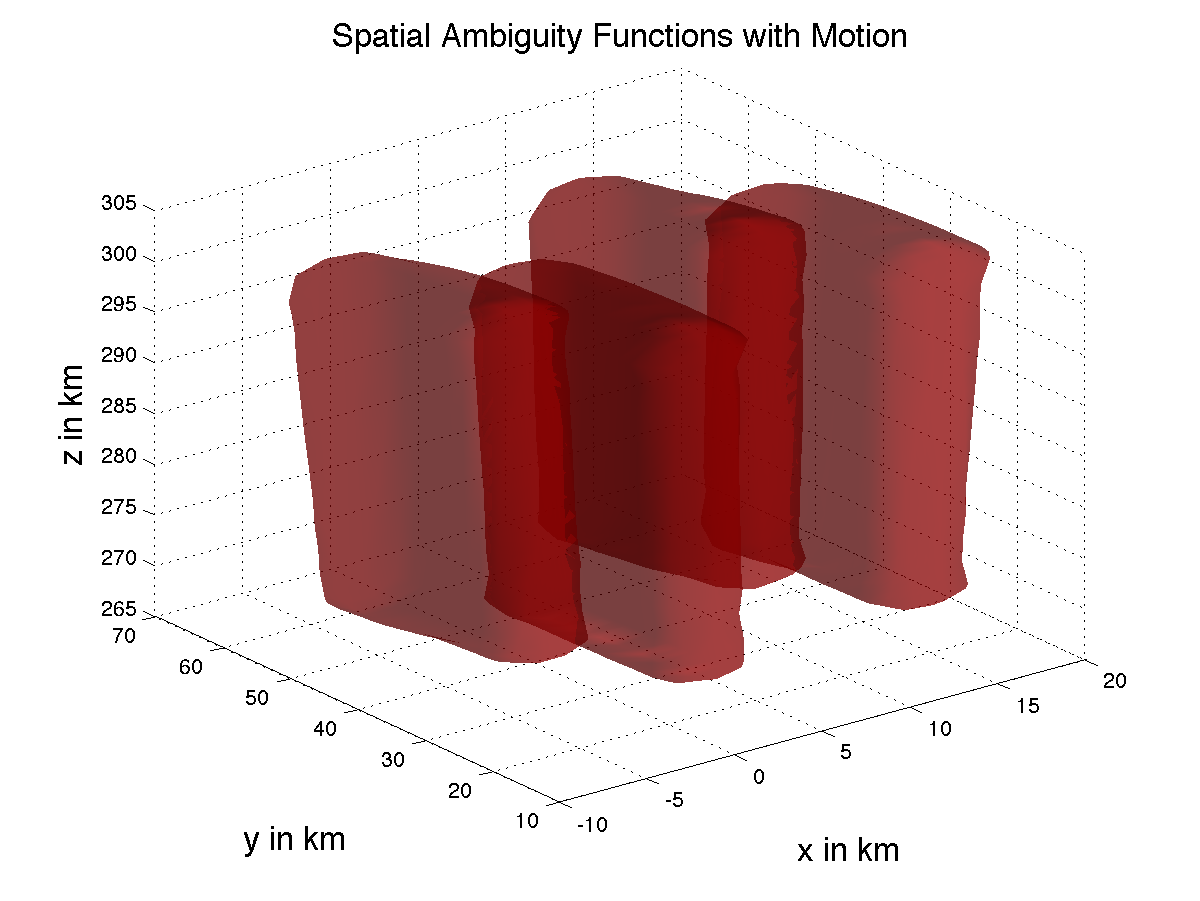
\includegraphics[width=5.5in]{spaceambmoving}
	\caption{Full Spatial Ambiguity Function With Motion}
	\label{fig:ambtime}
\end{figure}

The operator $A$ can be determined through knowledge of the radar system's beam pattern along with the experiments pulse pattern, integration time and velocity of the plasma. This velocity $\mathbf{v}$ can be estimated by taking taking measurements of the Doppler shift and using a methodology seen in \citep{butler:imagingfregiondrifts}. Once the operator has been determined standard processing techniques can be used as if the plasma is not moving.%debluring methods can be applied.

%%%%%%%%%%%%%% Simulation %%%%%%%%%%%%%%%%%%%%%%%%%%%%%%%%%%%%%

\section{Simulation}

In order to determine if it is possible to improve the resolution of ISR processing synthetic data was created using a known condition of a simulated ionosphere. The simulator creates data by deriving filters from the autocorrelation function and applying it to complex white Gaussian noise. In a sense every point in time and space noise plant and filter structure as in Figure \ref{fig:IQdiagram}. The data is then scaled and summed together according to its location in range and angle space to radar.

\begin{figure}[h!]
\centering
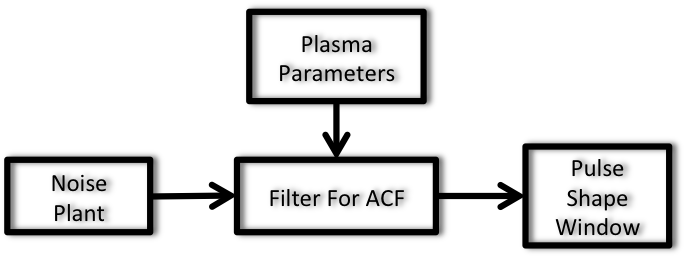
\includegraphics[width=3in]{diagrampart}
\caption{I/Q Simulator Diagram}
\label{fig:IQdiagram}
\end{figure}

After the IQ data has been created it is processed in to create an estimates of the ACF at desired points of space. This processing follows flow chart seen in Figure \ref{fig:chain}.

\begin{figure}[!t]
\centering
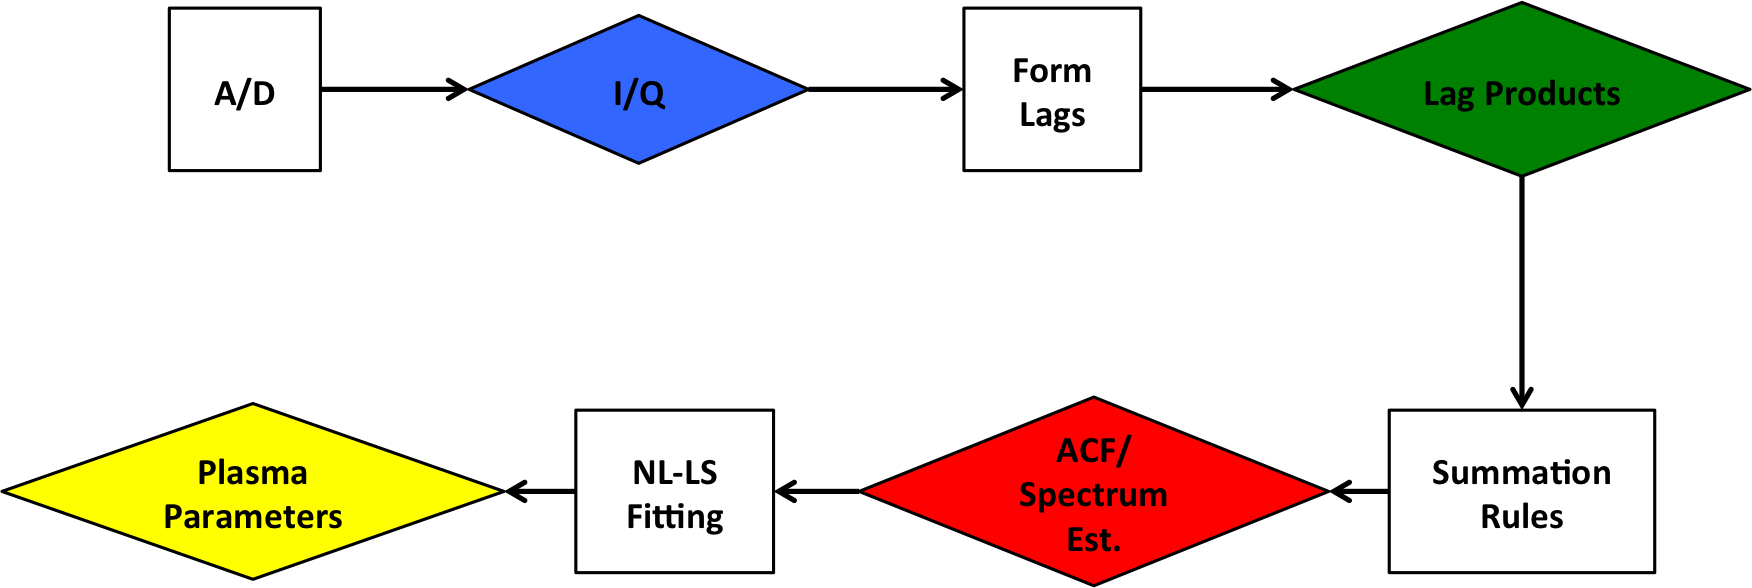
\includegraphics[width=6in]{datastackchain}
% where an .eps filename suffix will be assumed under latex, 
% and a .pdf suffix will be assumed for pdflatex; or what has been declared
% via \DeclareGraphicsExtensions.
\caption{ISR Processing Chain.}
\label{fig:chain}
\end{figure}

The sampled I/Q can be represented as $x(n) \in\mathbb{C}^N$ where $N$ is the number of samples in an inter pulse period.  At this point the first step in estimating the autocorrelation function is taken.  For each range gate $m\in 0,1,...M-1$ an autocorrelation is estimated for each lag of $l \in 0,1...,L-1$.  To get better statistics this operation is performed for each pulse $j\in 0,1,...J-1$ and then summed over the $J$ pulses.  The entire operation to form the initial estimate of $\hat{R}(m,l)$ can be seen in Equation \ref{lagpro}:

\begin{equation}
\label{lagpro}
\hat{R}(m,l) = \displaystyle\sum\limits_{j=0}^{J-1} x(m-\lfloor l/2\rfloor,j)x^*(m+\lceil l/2 \rceil,j).
\end{equation}


The case shown in Equation \ref{lagpro} is a centered lag product, other types of lag products calculations are available but generally a centered product is used. In the centered lag product case range gate index $m$ and sample index $n$ can be related by $m=n-\lfloor L/2\rfloor$ and the maximum lag and sample relation is $M=N-\lceil L/2 \rceil$. 

After the lag products have been formed an estimate of the noise correlation is subtracted out of $\hat{R}(m,l)$, which is defined as $\hat{R}_w(m,l)$:

\begin{equation}
\label{lagpro}
\hat{R}_w(m_w,l) = \displaystyle\sum\limits_{j=0}^{J-1} w(m_w-\lfloor l/2\rfloor,j)w^*(m_w+\lceil l/2 \rceil,j),
\end{equation}

\noindent where $w(n_w)$ is the background noise process of the radar.  Often the noise process is sampled during a calibration period for the radar when nothing is being emitted.  The final estimate of the autocorrelation function after the noise subtraction and summation rule will be represented by $\hat{R}_f(m,l)$. At this point a summation rule is applied and the data is sent off to be fit.

\begin{figure}
	\centering
	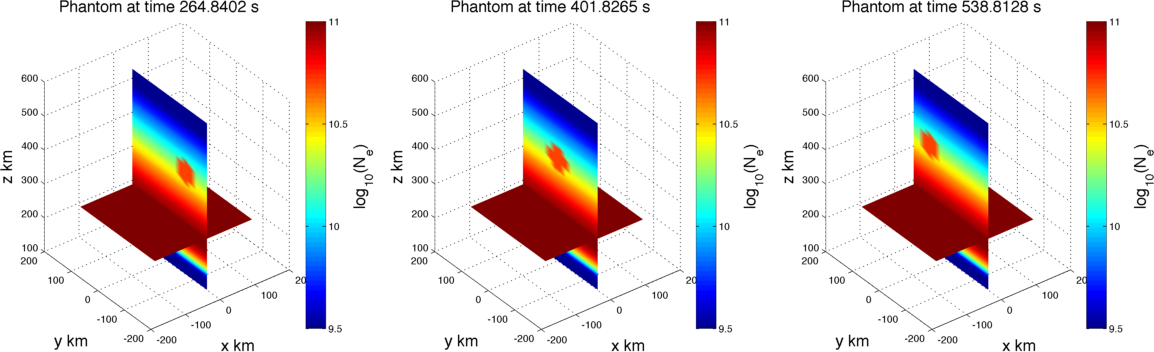
\includegraphics[width=6in]{phantom}
	\caption{Example images from phantom}	
	\label{fig:phantom}
\end{figure}

In order to demonstrate the blurring taking place from the motion of plasma a phantom ionosphere is created where a small plasma enhancement moves through the radar field of view. The background electron density varies in altitude as a Chapman function while the electron and ion temperature remains constant. This is done to avoid having to do full fit and thus only try to measure the electron density. Also estimates of the zeroth lag are only necessary. Added to this is a 35 km radius sphere of enhance electron density of about $5\times 10^{10} $ m$^{-3}$ centered at 400 km altitude moving at 500 m/s along the $\mathbf{y}$ direction. Images from this phantom can be seen in Figure \ref{fig:phantom}. 

Using the phantom we can see how just simply changing the integration time can impact the reconstruction. In Figure \ref{fig:variable} we can see a case were only 10 pulses are used for the reconstruction. This corresponds to an integration time of about 9 seconds using the 121 beam pattern. The enhancement can be seen with concentrated energy as it moves through the field of view. The problem is that there is a high amount of variance in the reconstruction. Figure \ref{fig:blurred} shows the reconstruction with 200 pulses, 3 minute integration time. The variability has been reduced but there is a large amount of blurring of the enhancement as it moves through the field of view. 
\begin{figure}
	\centering
	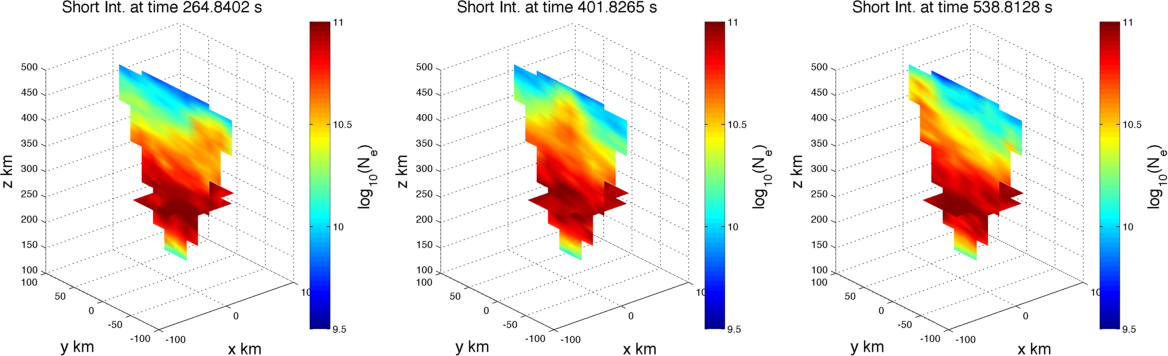
\includegraphics[width=6in]{variabledata}
	\caption{Example images from variable data}	
	\label{fig:variable}
\end{figure}


\begin{figure}
	\centering
	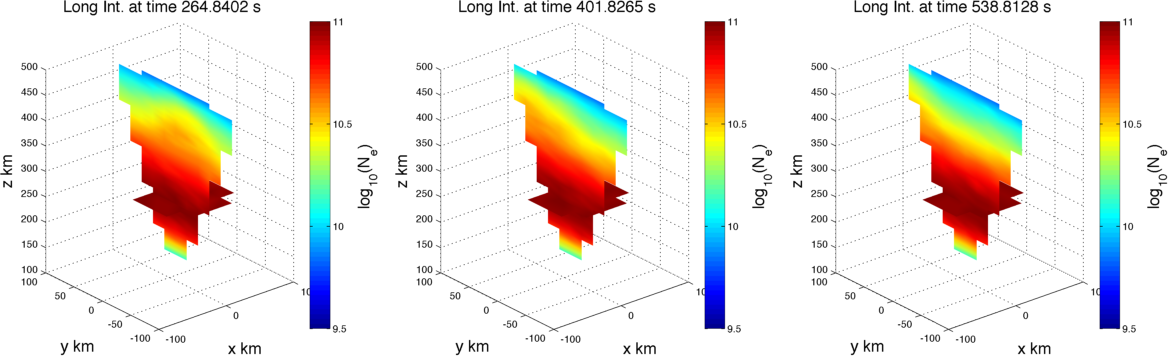
\includegraphics[width=6in]{blurreddata}
	\caption{Example images from blurred data}	
	\label{fig:blurred}
\end{figure}

In order to give a comparison a phantom was also created with no motion. This can be seen in Figure \ref{fig:phantomstat}. Images using the same integration time as in Figure \ref{variabledata} for the stationary phantom can be seen in \ref{fig:variablestat}. Another set of images using the longer integration time can be seen in \ref{fig:blurredstat}. These images show that the blurring is on the same order between both integration times.

\begin{figure}
	\centering
	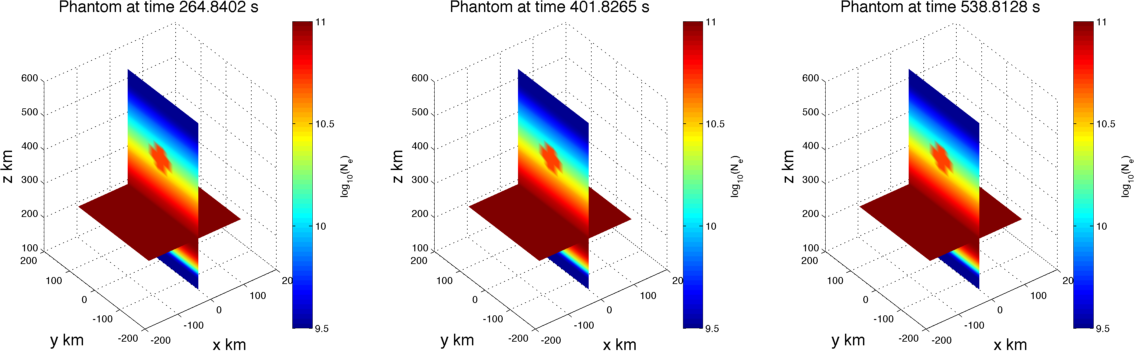
\includegraphics[width=6in]{phantomstation}
	\caption{Example images from phantom}	
	\label{fig:phantomstat}
\end{figure}

\begin{figure}
	\centering
	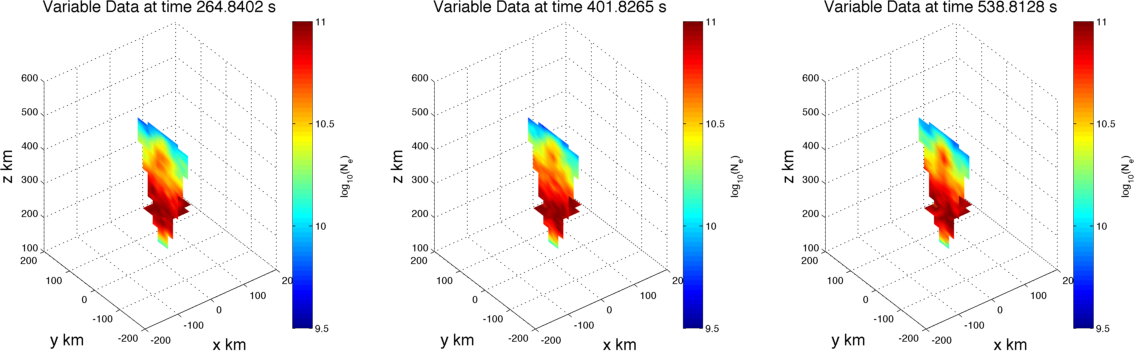
\includegraphics[width=6in]{variabledatastation}
	\caption{Example images from short integration of stationary plasma}	
	\label{fig:variablestat}
\end{figure}


\begin{figure}
	\centering
	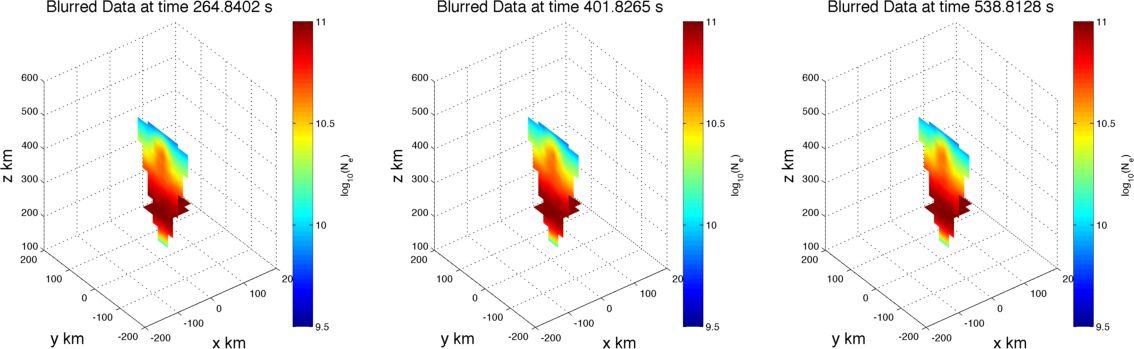
\includegraphics[width=6in]{blurreddatastation}
	\caption{Example images from longer integration time of stationary plasma}	
	\label{fig:blurredstat}
\end{figure}
%%%%%%%%%%%%%% Mitigation %%%%%%%%%%%%%%%%%%%%%%%%%%%%%%%%%%%%%

\section{Possible Mitigation Techniques}
There are a number of possible ways to remove the ISR operator function to the data. A relatively simply way to remove the problem is to process the data in the frame of reference of the plasma. This technique includes measuring the ion velocity of the plasma and then integrating the beams that the plasma is present in as it moves through the field of view.


In order to reconstruct the plasma parameters it is necessary to do some sort of regularization. There are two type of regularization that can be applied in this case the first is parameter based regularization, like full profile analysis, and the other is data based regularization. The term parameter based regularization in this case means applying constraints to the physical parameters that are often determined after fitting. This requires a large amount of calculation because the fitting and constraints are done in one step. Currently full profile analysis has only been applied along the range dimension and not in all three spatial dimensions. Extending this to three dimensions may make these algorithms computationally infeasible.

Data based regularization infers the application of constraints to the estimates of the autocorrelation functions. The constraints usually deal with how the data changes over time and space by constraining the energy of the ACFs or its derivative. This has an advantage of being more computationally tractable in that it is now a linear inverse problem. Using the ideas stated in this paper one can cast the reconstruction of the four dimensional function of the ACFs in these terms. The issue with doing this data based reconstruction is it is unknown how to constrain the reconstruction in the best way.
%%%%%%%%%%%%%% Conclusion %%%%%%%%%%%%%%%%%%%%%%%%%%%%%%%%%%%%

\section{Conclusion}
\bibliographystyle{BibTeX/agufull08}
\bibliography{BibTeX/litreview}

\begin{acknowledgments}
(Text here)
\end{acknowledgments}

\end{article}

\end{document}